\documentclass[../sparc.tex]{subfiles}
\graphicspath{{\subfix{../images/}}}
\begin{document}

%%%%%%%%%%%%%%%%%%%%%%%%%%%%%%%%%%%%%%%%%%%%%%%%%%%%%%%%%%%%%%%%%%%%%%%%%%%%%%%%
\section{Графика}
\index{Разработка игр!Графика}
\newglossaryentry{NPC}{name=NPC, description={Non-Playable Character --
    Не-игровой персонаж}}

%%%%%%%%%%%%%%%%%%%%%%%%%%%%%%%%%%%%%%%%%%%%%%%%%%%%%%%%%%%%%%%%%%%%%%%%%%%%%%%%
\subsection{Использование готовых символов}
\index{Программирование!Таблица символов}
\index{Разработка игр!Графика!Стандартные символы}

Компьютеры рассматривают символы также, как и всё остальное -- а именно в виде
чисел.  Каждому символу соответствует некий код, который компьютер запоминает и
обрабатывает, если мы просим сохранить символ в память или же вывести его на
экран.

\note{ Одной из простейших форм кодирования символов является таблица ASCII
  (American Standard Code for Information Interchange), которая описывает
  символы с кодами от нуля до 127 включительно.  В современных операционных
  системах для обеспечения поддержки различных языков вместо ASCII используется
  кодировка Unicode, в которой размер таблицы намного больше и включает в себя
  символы большинства народов мира.  Тем не менее, Unicode сохраняет обратную
  совместимость с ASCII и первые 128 символов в Unicode повторяют символы из
  таблицы ASCII.}

В текстовых ЖК-дисплеях есть встроенная таблица символов, согласно которой
дисплей отображает символы.  Набор этих символов различается в зависимости от
модели дисплея, поэтому рекомендуется поискать таблицу символов именно для
вашего дисплея.

Например, во многих дисплеях символ с кодом 255 (\texttt{0xFF} в
шестнадцатиричной системе) обозначает полностью закрашенный блок.  Для того,
чтобы использовать данный символ в проекте, удобно завести для него константу,
обозначающую данный игровой ``объект'':

\begin{minted}{cpp}
  const char WALL = 0xFF; // Код символа
\end{minted}

Обратите внимание, что код символа указывается без кавычек, так как мы явно
указываем номер символа в таблице, а не его графическое представление.

После того, как мы создали констатну для символа, мы можем выводить его в коде
программы следующим образом:

\begin{minted}{cpp}
  void loop() {
    lcd.setCursor(0, 0);
    lcd.print(WALL);
  }
\end{minted}

%%%%%%%%%%%%%%%%%%%%%%%%%%%%%%%%%%%%%%%%%%%%%%%%%%%%%%%%%%%%%%%%%%%%%%%%%%%%%%%%
\subsection{Создание собственных символов}
\index{Разработка игр!Графика!Создание символов}

Несмотря на то, что дисплей в нашем проекте используется текстовый, и он не даёт
нам возможности рисовать произвольные рисунки в любом месте экрана, нам доступна
возможность создавать собственные символы.  Эти символы затем можно отображать в
клетках дисплея.

Размер клетки на нашем дисплее составляет 8х5 пикселей (8 строк на 5 столбцов.)
Схематически это можно визуализировать, как показано на
рис. \ref{fig:game-dev-char}.

\begin{figure}[ht]
  \centering
  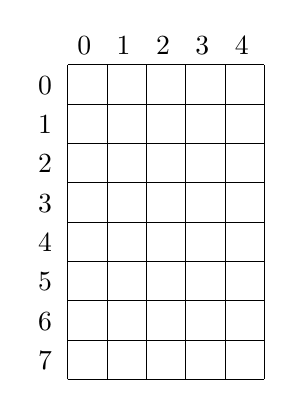
\begin{tikzpicture}
    \draw[step=0.5cm,black,very thin] (-2.5, -4) grid (0, 0);
    \foreach[count=\n from 0] \x in {-2.5, -2.0, ..., -0.5} {
      \draw (\x cm, 0) node[anchor=south west] {$\n$};
    }
    \foreach[count=\n from 0] \y in {-0.5, -1.0, ..., -4} {
      \draw (-3.0, \y) node[anchor=south west] {$\n$};
    }
  \end{tikzpicture}
  \caption{Схематическое изображение клетки, в которой отрисовывается символ.}
  \label{fig:game-dev-char}
\end{figure}

На дисплее 4 строки на 20 столбцов всего 80 таких клеток, показанных на рис.
\ref{fig:game-dev-char}.

Каждый пиксель описывается одним битом. Единица означает, что пиксель закрашен,
ноль означает, что пиксель не закрашен. Например, строчка, показанная на рис.
\ref{fig:game-dev-char-symbol-encoding}, может быть описана, как
\texttt{0b01010}.

\note{ Обратите внимание, что числа, начинающиеся с префикса \texttt{0b} (символ
  нуля и английской буквы ``b''), записаны напрямую в двоичном виде.  Не стоит
  забывать, что компьютер \emph{все} данные, которые мы сохраняем в памяти,
  хранит в двоичном виде; задавая префикс перед числом, мы лишь меняем формат
  записи числа, а не формат хранения.  Из других префиксов можно назвать
  \texttt{0x} (ноль-икс), позволяющий указывать шестнадцатиричные числа
  (например \texttt{0xFF}) и префикс \texttt{0} (ноль), позволяющий указывать
  восьмеричные числа. }

\begin{figure}[ht]
  \centering
  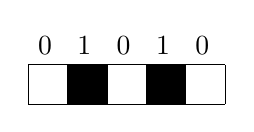
\begin{tikzpicture}
    \draw[step=0.5cm,black,very thin] (-2.5, -0.5) grid (0, 0);
    \fill[black] (-2.0, 0) rectangle (-1.5, -0.5);
    \fill[black] (-1.0, 0) rectangle (-0.5, -0.5);
    \foreach \x/\n in {-2.5/0, -2.0/1, -1.5/0, -1.0/1, -0.5/0} {
      \draw (\x cm, 0) node[anchor=south west] {$\n$};
    }
  \end{tikzpicture}
  \caption{Кодирование пикселей в одной строке символа.}
  \label{fig:game-dev-char-symbol-encoding}
\end{figure}

Одна строка символа кодируется одним байтом информации (восемью битами) из
которых фактически используется только пять младших бит.  Всего таких строк 8
штук, и для их хранения нам нужен массив на восемь байт.

Пример отрисовки человечка:

\begin{minted}{cpp}
  byte player_image[8] = {
    0b01110,
    0b01110,
    0b00100,
    0b01110,
    0b10101,
    0b01110,
    0b01010,
    0b01010
  };
\end{minted}

Визуальное представление данного символа:

\begin{figure}[ht]
  \centering
  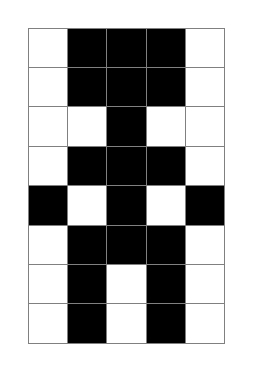
\begin{tikzpicture}
    %% 0
    \fill[black] (-2.0, 0) rectangle (-0.5, -1.0);
    %% 2
    \fill[black] (-1.0, -1.0) rectangle (-1.5, -1.5);
    %% 3
    \fill[black] (-0.5, -1.5) rectangle (-2.0, -2.0);
    %% 4
    \fill[black] (-2.0, -2.0) rectangle (-2.5, -2.5);
    \fill[black] (-1.5, -2.0) rectangle (-1.0, -2.5);
    \fill[black] (-0.5, -2.0) rectangle (-0.0, -2.5);
    %% 5
    \fill[black] (-0.5, -2.5) rectangle (-2.0, -3.0);
    %% 6
    \fill[black] (-2.0, -3.0) rectangle (-1.5, -3.5);
    \fill[black] (-1.0, -3.0) rectangle (-0.5, -3.5);
    %% 7
    \fill[black] (-2.0, -3.5) rectangle (-1.5, -4.0);
    \fill[black] (-1.0, -3.5) rectangle (-0.5, -4.0);
    \draw[step=0.5cm,gray,very thin] (-2.5, -4.0) grid (0, 0);
  \end{tikzpicture}
  \caption{Изображение игрока.}
  \label{fig:game-dev-char-symbol-example}
\end{figure}

Можно рисовать подобные изображения на тетрадном листе в клетку, и потом вручную
переводить это в программный код.  Само собой, программисты уже автоматизировали
этот процесс, и есть готовые online-ресурсы для рисования символов и
автоматической генерации программного кода.  Вот один из них:
\url{https://omerk.github.io/lcdchargen/}

После того, как символ нарисован, его надо прописать в память дисплея, чтобы мы
могли его нарисовать.  Из встроенной таблицы символов нам обычно доступны коды
символов от 0 до 7 включительно, что даёт возможность записать 8 собственных
символов в память.  Остальные символы во встроенной таблице переписать нельзя.

Для того, чтобы прописать символ в память, нам нужно использовать специальную
функцию \texttt{createChar}, в которую мы должны передать код символа и желаемое
его представление на дисплее, заданное через массив.  Для задания кода символа
удобно использовать константы типа \texttt{char}, поэтому мы создадим константу
\texttt{PLAYER} для нашего игрока:

\begin{minted}{cpp}
  const char PLAYER = 0; // Код символа
  // Визуальное представление символа.
  byte player_image[8] = {
    0b01110,
    0b01110,
    0b00100,
    0b01110,
    0b10101,
    0b01110,
    0b01010,
    0b01010
  };
\end{minted}

Затем в \texttt{setup} пропишем символ в память дисплея:

\begin{minted}{cpp}
  void setup() {
    lcd.init();
    lcd.backlight();

    // Запись символа в память дисплея:
    lcd.createChar(PLAYER, player_image);
  }
\end{minted}

После этого мы можем вывести символ на ЖК-дисплей просто вызвав функцию
\texttt{print}, передав в неё нашу константу \texttt{PLAYER}:

\begin{minted}{cpp}
  void loop() {
    lcd.setCursor(0, 0);
    lcd.print(PLAYER);
  }
\end{minted}

%%%%%%%%%%%%%%%%%%%%%%%%%%%%%%%%%%%%%%%%%%%%%%%%%%%%%%%%%%%%%%%%%%%%%%%%%%%%%%%%
\subsection{Задачи}
\begin{enumerate}
\item Добавьте символы для не-игрового персонажа (\gls{NPC}) и для некоторого
  собираемого предмета.
\end{enumerate}

\end{document}
